% !TeX spellcheck = en_GB

As we mentioned several times before in this thesis, biological neural networks are dynamical systems.
Taken at face value, this assertion is a gross understatement---of course, just like all other physical systems, biological systems evolve through time and are thus \enquote{dynamic}.
However, dynamics are of special interest when studying nervous systems.
At the lowest level---and as we hope to convince the reader in this chapter---neural dynamics play a critical role in biological computation.
Simultaneously, at the highest level, dynamics determine the overall ability of an organism to survive.
Variations in response-time on the order of milliseconds can decide over life and death, 
as avid viewers of nature documentaries and motor vehicle operators will surely attest.

From the perspective of classical computer engineering, it may almost seem implausible that a biological system should be capable of rapid coordinated action---particularly taking into account that the elements that make up nervous systems compute asynchronously and possess strong intrinsic dynamics.
After all, when constructing artificial computers, asynchronicity and dynamics are annoyances that engineers must work around.
Typical microprocessors spend a sizeable portion of their energy budget on distributing clock signals \citep[e.g.,][]{zhang2008injectionlocked}, and most digital circuits are meticulously engineered to switch between clearly interpretable voltage states as quickly as possible \citep[e.g.,][Chapter~4]{weste2011cmos}.
Similarly, on an algorithmic level, neurons in artificial neural networks are assumed compute instantly, while time progresses synchronously in discrete steps.

This juxtaposition of artificial and biological systems gives rise to an old, but still common (and rather subtle) mis\-cha\-rac\-te\-ri\-sa\-tion---namely, the idea that biological information processing is slow and that, compared to digital computers, biological brains compensate for their slowness with massive parallelism (see for example \cite{vonneumann1958computer}, pp.~50f).
Of course, this statement is true in some respect.
For example, signal propagation in electronic circuits is between six and eight orders of magnitudes faster than axonal action potential propagation.%
\footnote{Electrical signals travel at about two thirds of the speed of light along conductors (i.e., about \SI{200e6}{\metre\per\second}), whereas axonal action potential propagation can be as slow as \SI{1}{\metre\per\second} and reaches up to \SI{100}{\metre\per\second}.}
Still, comparing digital computers and neural networks without fully understanding the high-level computational function of individual neurons amounts to guesswork; simply stating that neurons and synapses are \enquote{slow} misses the point.

A central hypothesis of this chapter is that the processes that generate neural dynamics are a crucial for the computations performed by biological system.
Neural dynamics are \emph{responsible} for high-level functions such as interpreting visual motion, forming working memory, and generating motor trajectories.
In a nutshell, computations that depend on the history of a signal on short time-scales is possible \emph{because} of (and not despite) information about the past signal history being implicitly stored in the \enquote{slow} temporal dynamics.

It should be emphasised that we are by no means suggesting that dynamical system theory is the \emph{primary} paradigm by which cognitive scientists and artificial intelligence researchers should model cognitive systems.



\subsubsection{Goal of this chapter}

The goal of this chapter to convince the reader that this interpretation of neural dynamics can indeed be used to 

\subsubsection{Prior work}

\begin{figure}
	\centering
	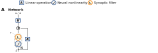
\includegraphics{media/chapters/04_temporal_tuning/nef_principle_three_examples_network.pdf}%
	\kern-124mm\includegraphics{media/chapters/04_temporal_tuning/nef_principle_three_examples.pdf}
	\caption[Approximating arbitrary dynamics using the NEF dynamics principle]{Approximating arbitrary dynamics using the NEF dynamics principle.
	\textbf{(A)} Simplified network architecture; encoders and decoders are not shown (see \cref{fig:nef_dynamics_neurons_a} for the full network).
	Either $u(t)$ or $\dot u(t)$ is passed into the network; $\mat{A'}$ and $\mat{B'}$ are the LTI system matrices compensating for the synaptic filter with time-constant $\tau$ (eq.~\ref{eqn:nef_transform_a_b}).
	\textbf{(B)} Without the recurrent connection (i.e., $\mat{A'} = 0$, $\mat{B'} = 1$), the system acts as a low-pass filter.
	\textbf{(C)} Implementing an integrator ($\mat{A} = 0$, $\mat{B} = 1$).
	\textbf{(D)} With access to the differential $\dot u(t)$, the integrator can be used to construct a pass-through.
	}
\end{figure}

The work in this chapter can primarily be seen as a generalisation of the NEF dynamics principle.
Recall that the dynamics principle (\Cref{chp:nef_dynamics}) states that recurrent connections within a spiking neural network can be used to approximate \emph{any} dynamical system of the form $\dot{x}(t) = f(x(t), u(t), t)$.
Examples include approximating an integrator $\dot{x}(t) = u(t)$, or a low-pass filter $\bar \tau \dot{x}(t) = u(t) - x(t)$.
Notably, the time-constant of the simulated low-pass filter $\bar \tau$ can be shorter than the synaptic time constant $\tau$ of the underlying system.
Assuming that we have access to the differential $\dot u(t)$, we can use the integrator to compensate for the neural dynamics altogether.

In contrast to artificial neural networks, and as we discussed before, the individual computing elements that make up biological neural networks 

The dynamics of the individual components that make up a nervous system are not merely by accident, 

% Dynamics of the individual elements are not merely an accident
% Form working memories
% Stream-processing information in real-time

As we have discussed several times before, biological neural systems are \emph{inherently} continuous dynamical systems that are based on asynchronous computing elements.

Biological neural networks are continuous dynamical systems that are based on asynchronous computing elements.
This is in contrast to artificial neural networks, which are typically engineered to work with relatively coarse timesteps on a synchronous computing substrate.

So far, we have mostly ignored network-level dynamics.
Of course, our analysis of \emph{individual neurons} in the \nlif family critically relied on harnessing the subthreshold dynamics of the passive dendrites for computation.
However, when constructing \emph{networks}, we characterised these neurons in terms of a time-averaged response curve $\mathscr{G}[\vec g]$ (\Cref{sec:nlif_derive_h}) and did not account for the filter-properties of the dendrites (\Cref{sec:nlif_subth_properties}).

The goal of this chapter is to present techniques for harnessing the dynamical properties of spiking neural networks for computing time-dependent functions, that is, functions that do not only depend on a current system state $\vec x \in \mathbb{R}^d$, but on a \emph{signal} $\mathfrak{x}(t) : \mathbb{R}^- \longrightarrow \mathbb{R}^d$, where $t = 0$ corresponds to the current point in time, and $t < 0$ references the signal history.

While the focus of this chapter will not be on multi-channel neurons such as \nlif neurons, ...

\begin{itemize}
	\item We mostly focus on linear dynamics
\end{itemize}

NEF Dynamics Principle: Separation of dynamics and represented quantities.
Can solve for dynamics by sampling, do not require a dynamical system description: this is a key feature of the NEF!

\begin{Notation}
In this chapter, we sometimes use Fraktur letters (e.g., $\mathfrak{a}$, $\mathfrak{b}$, \textellipsis) to convey that the mathematical objects we are referring to are now \emph{functions} over time.
That is, we write the stimulus history as $\vec{\mathfrak{x}}(t)$ instead of $\vec x(t)$.
Note that $\vec{\mathfrak{x}}(t)$ refers to the result of evaluating the function $\vec{\mathfrak{x}}$ at a specific point in time $t$, whereas $\vec{\mathfrak{x}}$ refers to the function object as a whole.
In other words, $\vec{\mathfrak{x}}$ is a map $\mathbb{R} \longrightarrow \mathbb{R}^d$, whereas $\vec{\mathfrak{x}}(t)$ is simply an element in $\mathbb{R}^d$.
This distinction is important when expressing operations on functions, such as convolution.
We furthermore assume in most of our definitions that $t = 0$ corresponds to the current point in time.
Since nervous systems usually do not have access to future events, the stimulus history $\vec{\mathfrak{x}}(t)$ only needs to be defined for $t \leq 0$.
\end{Notation}
